\documentclass[11pt,a4paper]{article}

\usepackage[utf8]{inputenc}
\usepackage[T1]{fontenc}
\usepackage{lmodern}
\usepackage{amsmath,amssymb}
\usepackage{booktabs}
\usepackage{graphicx}
\usepackage[ruled,vlined,linesnumbered]{algorithm2e}
\usepackage{hyperref}
\usepackage[margin=2.5cm]{geometry}
\usepackage{tikz}
\usepackage{pgfplots}
\pgfplotsset{compat=1.18}
\usetikzlibrary{arrows.meta,positioning,patterns,decorations.markings}

\title{Ogun: Spatial Layout Generation via Sequential Logit Dynamics\\on Potential Games}
\author{Elias Vahlberg}
\date{March 2026}

\begin{document}
\maketitle

% ────────────────────────────────────────────────────────────────
\begin{abstract}
We present Ogun, a deterministic spatial layout algorithm that places nodes and
routes edges on a 2D grid by modeling placement as a potential game solved via
sequential logit dynamics. Agents arrive in a fixed order, evaluate a potential
function $\Phi$ encoding attraction, repulsion, and configurable kernel terms
over every grid cell, then commit irrevocably to a position sampled from the
Boltzmann distribution $P(p) \propto \exp(\beta \cdot \Phi(p))$. Edges are
routed during placement using congestion-aware Dijkstra and refined
post-placement via PathFinder negotiation (rip-up-and-reroute). The inverse
temperature $\beta$ acts as a single control parameter governing output
character, from near-random ($\beta \to 0$) to near-optimal ($\beta \to
\infty$). We describe the algorithm, analyze its complexity, and demonstrate its
application to procedural city generation.

\medskip
\noindent\textbf{Keywords:} procedural generation, potential games, logit
dynamics, spatial layout, pathfinding, negotiation routing
\end{abstract}

% ────────────────────────────────────────────────────────────────
\section{Introduction}

Procedural generation of structured 2D layouts (cities, dungeons, circuit
boards) requires solving two coupled problems simultaneously: \emph{placement}
(where to put things) and \emph{routing} (how to connect them). Classical
approaches treat these as separate optimization passes: force-directed placement
followed by maze routing~\cite{mcmurchie1995}. This decoupling loses
information; placement decisions made without routing awareness produce layouts
that are difficult or impossible to route efficiently.

Ogun couples placement and routing into a single sequential process. Each agent
(node) observes the current state, including routes already laid, before
choosing its position. The placement decision is formalized as a potential game
where the potential function $\Phi$ encodes both local quality (overlap,
repulsion, attraction to neighbors) and global structure (boundary affinity,
terrain compatibility). The Boltzmann sampling mechanism provides a principled
interpolation between greedy optimization and stochastic exploration, controlled
by a single parameter $\beta$.

The algorithm draws on two traditions: \emph{logit dynamics} from evolutionary
game theory~\cite{blume1993}, where agents update strategies with noise
proportional to $1/\beta$; and \emph{negotiation-based routing} from electronic
design automation~\cite{mcmurchie1995}, where competing routes iteratively
resolve conflicts through congestion penalties. The combination produces layouts
that are structured yet organic, well-suited to procedural content generation
for games.

The name \emph{Ogun} comes from the Yoruba deity of iron, metalwork, and
pathfinding, a god who cleared the first roads through primordial wilderness.

% ────────────────────────────────────────────────────────────────
\section{Problem Formulation}

\subsection{Definitions}

Let $G = (V, E)$ be a weighted undirected graph where each node $v_i \in V$ has
a footprint radius $r_i \in \mathbb{N}$ and each edge $e_k = (v_i, v_j, w_k)$
has a weight $w_k > 0$ encoding connection importance.

Let $S = (W, H, \mathcal{O})$ be a spatial domain: a $W \times H$ integer grid
with obstacle set $\mathcal{O} \subset [0,W) \times [0,H)$. Optionally, $S$
carries a routing cost grid $\rho: [0,W) \times [0,H) \to \mathbb{R}^+$
(default $\rho \equiv 1$).

\subsection{Output}

A \emph{layout} $L$ consists of:
\begin{itemize}
    \item A position map $\pi: V' \to S$ for placed nodes $V' \subseteq V$
    \item A path map $\gamma: E' \to S^*$ for routed edges $E' \subseteq E$
    \item A score breakdown $(s_\text{pe}, s_\text{acc}, s_\text{cong}, s_\text{vr}) \in [0,1]^4$
\end{itemize}

\subsection{Objective}

Maximize the composite score $s = \frac{1}{4}(s_\text{pe} + s_\text{acc} +
s_\text{cong} + s_\text{vr})$ subject to:
\begin{enumerate}
    \item No two node footprints overlap
    \item No node footprint intersects an obstacle
    \item All paths are 4-connected and avoid obstacles and footprints (except at endpoints)
\end{enumerate}

The parameter $\beta$ does not appear in the objective; it controls the
\emph{stochasticity} of the search, not the target.

% ────────────────────────────────────────────────────────────────
\section{Algorithm Overview}

Ogun proceeds in two phases. Phase~1 places nodes sequentially with
congestion-aware routing after each placement. Phase~2 refines all routes via
PathFinder negotiation.

\begin{algorithm}[H]
\SetAlgoLined
\KwIn{Graph $G=(V,E)$, Space $S$, Config $(\beta, \text{seed}, K, \rho)$}
\KwOut{Layout $L$}
$\text{rng} \gets \text{ChaCha8}(\text{seed})$\;
\ForEach{node $v_i$ in arrival order}{
    \ForEach{valid position $p \in S$}{
        $u_i(p) \gets \Phi(p, v_i, \text{state})$\tcp*{Evaluate potential}
    }
    $p^* \sim \text{Boltzmann}(\{u_i(p)\}, \beta, \text{rng})$\tcp*{Sample}
    Place $v_i$ at $p^*$; block footprint\;
    \ForEach{edge $(v_i, v_j)$ where $v_j$ is placed}{
        $\gamma_{ij} \gets \text{DijkstraCongestion}(p^*, \pi(v_j), S)$\;
    }
}
\For{$t = 1$ \KwTo $T_\text{neg}$}{
    \ForEach{edge $e_k$ sorted by weight descending}{
        Rip up $\gamma_k$; reroute via Dijkstra with updated congestion\;
    }
    \If{no shared cells}{break\;}
    Update history penalties on congested cells\;
}
Score layout and return $L$\;
\caption{Ogun: Sequential Logit Dynamics with Negotiated Routing}
\end{algorithm}

% ────────────────────────────────────────────────────────────────
\section{Potential Function}

The potential $\Phi(p, v_i, \text{state})$ decomposes into four terms:

\begin{equation}
\Phi(p, v_i) = \underbrace{-\sum_{j \in N(i)} w_{ij} \cdot d(p, \pi(v_j))}_{\text{attraction}}
+ \underbrace{\sum_{j \in \text{placed}} \frac{k_r \cdot m_{ij}}{d^2(p, \pi(v_j))}}_{\text{repulsion}}
+ \underbrace{\Phi_\text{boundary}(p, v_i)}_{\text{affinity}}
+ \underbrace{B(p)}_{\text{cell bonus}}
\end{equation}

where $N(i)$ is the set of placed neighbors of $v_i$, $k_r$ is the global
repulsion constant, $m_{ij}$ is a per-pair repulsion multiplier (default 1),
and $d(\cdot,\cdot)$ is Euclidean distance.

\begin{figure}[ht]
\centering
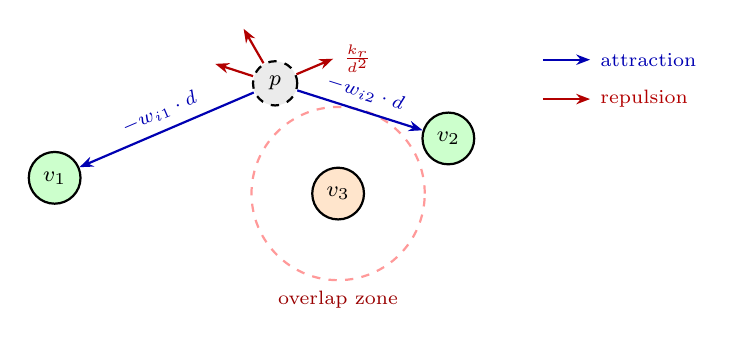
\begin{tikzpicture}[
    node/.style={circle, draw, thick, minimum size=18pt, font=\footnotesize},
    candidate/.style={circle, draw, thick, dashed, minimum size=14pt,
                      fill=black!8, font=\footnotesize},
    attract/.style={-{Stealth[length=5pt]}, thick, blue!70!black},
    repel/.style={-{Stealth[length=5pt]}, thick, red!70!black},
]
% Placed nodes
\node[node, fill=green!20] (A) at (0, 0) {$v_1$};
\node[node, fill=green!20] (B) at (5, 0.5) {$v_2$};
\node[node, fill=orange!20] (C) at (3.6, -0.2) {$v_3$};

% Candidate position
\node[candidate] (P) at (2.8, 1.2) {$p$};

% Overlap zone around C (shown as dashed circle)
\draw[red!40, dashed, thick] (C) circle (1.1cm);
\node[font=\scriptsize, red!60!black] at (3.6, -1.55) {overlap zone};

% Attraction arrows (from p toward connected neighbors)
\draw[attract] (P) -- node[above, font=\scriptsize, sloped] {$-w_{i1} \cdot d$} (A);
\draw[attract] (P) -- node[above, font=\scriptsize, sloped] {$-w_{i2} \cdot d$} (B);

% Repulsion arrows (force on p, pointing away from each placed node)
% From v1(0,0): direction through p(2.8,1.2) ≈ 23°
\draw[repel] (P) -- ++(23:0.8)
    node[right, font=\scriptsize] {$\frac{k_r}{d^2}$};
% From v2(5,0.5): direction through p(2.8,1.2) ≈ 162°
\draw[repel] (P) -- ++(162:0.8);
% From v3(3.6,-0.2): direction through p(2.8,1.2) ≈ 120°
\draw[repel] (P) -- ++(120:0.8);

% Legend
\draw[attract] (6.2, 1.5) -- ++(0.6, 0)
    node[right, font=\scriptsize] {attraction};
\draw[repel] (6.2, 1.0) -- ++(0.6, 0)
    node[right, font=\scriptsize] {repulsion};
\end{tikzpicture}
\caption{Forces acting on a candidate position $p$ for a new node $v_i$.
Blue arrows show attraction toward connected, already-placed neighbors
($v_1$, $v_2$). Red arrows show repulsion pushing $p$ away from all placed
nodes. If $p$ falls within the overlap zone of any placed node (dashed circle
around $v_3$), the position is rejected.}
\label{fig:potential}
\end{figure}

\paragraph{Overlap rejection.} If $d(p, \pi(v_j)) < r_i + r_j$ for any placed
node $v_j$, or if $p \in \mathcal{O}$, the position is rejected ($\Phi =
\bot$).

\paragraph{Repulsion cutoff.} Contributions where $d^2 > 100 k_r$ are skipped,
bounding the repulsion pass at $O(n_\text{nearby})$ rather than $O(n)$.

\paragraph{Boundary affinity.} For nodes with affinity $a_i \neq 0$:
\begin{equation}
\Phi_\text{boundary}(p, v_i) = a_i \cdot \left(1 - \frac{d_\text{edge}(p)}{\lfloor \min(W,H)/2 \rfloor}\right)
\end{equation}
where $d_\text{edge}(p) = \min(p_x, W{-}1{-}p_x, p_y, H{-}1{-}p_y)$.

\paragraph{Cell bonus.} An optional grid $B: S \to \mathbb{R}$ adds per-cell
utility for terrain compatibility or zoning preferences.

% ────────────────────────────────────────────────────────────────
\section{Boltzmann Sampling}

Given candidate utilities $\{u_1, \ldots, u_m\}$, the agent selects position
$p_j$ with probability:
\begin{equation}
P(p_j) = \frac{\exp(\beta \cdot u_j)}{\sum_{k=1}^{m} \exp(\beta \cdot u_k)}
\end{equation}

The log-sum-exp trick prevents overflow: subtract $u_{\max} = \max_k u_k$
before exponentiation. Sampling uses inverse CDF with a single uniform draw,
requiring no weight vector allocation (two-pass streaming).

As $\beta \to \infty$, sampling converges to $\arg\max$; as $\beta \to 0$,
sampling becomes uniform. This provides a smooth interpolation between greedy
placement and random exploration.

\begin{figure}[ht]
\centering
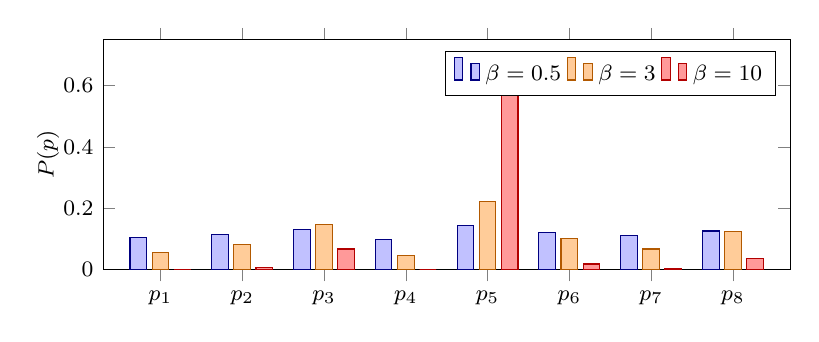
\begin{tikzpicture}
\begin{axis}[
    width=0.85\textwidth, height=4.5cm,
    ybar, bar width=6pt,
    ymin=0, ymax=0.75,
    symbolic x coords={$p_1$,$p_2$,$p_3$,$p_4$,$p_5$,$p_6$,$p_7$,$p_8$},
    xtick=data,
    ylabel={$P(p)$},
    ylabel style={at={(-0.05,0.5)}},
    legend style={at={(0.98,0.95)}, anchor=north east, font=\footnotesize,
                  legend columns=3},
    legend cell align={left},
    every axis plot/.append style={fill opacity=0.8},
    tick label style={font=\footnotesize},
    label style={font=\footnotesize},
]
% Utilities: [0.3, 0.5, 0.8, 0.2, 1.0, 0.6, 0.4, 0.7]
% Low beta = 0.5 (nearly uniform)
\addplot[fill=blue!30, draw=blue!50!black] coordinates {
    ($p_1$,0.104) ($p_2$,0.115) ($p_3$,0.131)
    ($p_4$,0.099) ($p_5$,0.145) ($p_6$,0.121)
    ($p_7$,0.110) ($p_8$,0.126)
};
% Medium beta = 3 (peaked)
\addplot[fill=orange!50, draw=orange!70!black] coordinates {
    ($p_1$,0.055) ($p_2$,0.083) ($p_3$,0.148)
    ($p_4$,0.045) ($p_5$,0.222) ($p_6$,0.100)
    ($p_7$,0.067) ($p_8$,0.124)
};
% High beta = 10 (spike at argmax)
\addplot[fill=red!50, draw=red!70!black] coordinates {
    ($p_1$,0.001) ($p_2$,0.007) ($p_3$,0.067)
    ($p_4$,0.000) ($p_5$,0.665) ($p_6$,0.018)
    ($p_7$,0.002) ($p_8$,0.037)
};
\legend{$\beta = 0.5$, $\beta = 3$, $\beta = 10$}
\end{axis}
\end{tikzpicture}
\caption{Effect of inverse temperature $\beta$ on position selection
probability for eight candidate positions with varying utility. At low $\beta$,
the distribution is nearly uniform (exploratory). At high $\beta$, probability
concentrates on the highest-utility position $p_5$ (greedy). Intermediate
$\beta$ balances exploration and exploitation.}
\label{fig:boltzmann}
\end{figure}

% ────────────────────────────────────────────────────────────────
\section{Routing}

\subsection{Phase 1: Congestion-Aware Dijkstra}

After each node placement, edges to already-placed neighbors are routed via
Dijkstra on the 4-connected grid. The edge cost at cell $p$ is:
\begin{equation}
C(p) = \rho(p) \cdot (1 + h(p)) \cdot (1 + s(p))
\end{equation}
where $\rho(p)$ is the base routing cost, $h(p)$ is accumulated history
penalty, and $s(p)$ is the current sharing count (number of routes using $p$).

Cells blocked by node footprints are impassable except at route endpoints.

\subsection{Phase 2: PathFinder Negotiation}

After all nodes are placed, routes are iteratively ripped up and rerouted to
resolve congestion, following the PathFinder
algorithm~\cite{mcmurchie1995}:

\begin{enumerate}
    \item For each edge (sorted by weight descending): remove its path from the
    sharing grid, reroute via Dijkstra with current congestion costs, add the
    new path back.
    \item If no cell has $s(p) > 1$, terminate (convergence).
    \item Otherwise, increment history: $h(p) \mathrel{+}= \delta$ for all $p$
    where $s(p) > 1$.
    \item Repeat for up to $T_\text{neg}$ iterations.
\end{enumerate}

Higher-weight edges are rerouted first, giving important connections priority
over minor ones. The history penalty ensures that persistently congested cells
become increasingly expensive, forcing routes to find alternatives.

\begin{figure}[ht]
\centering
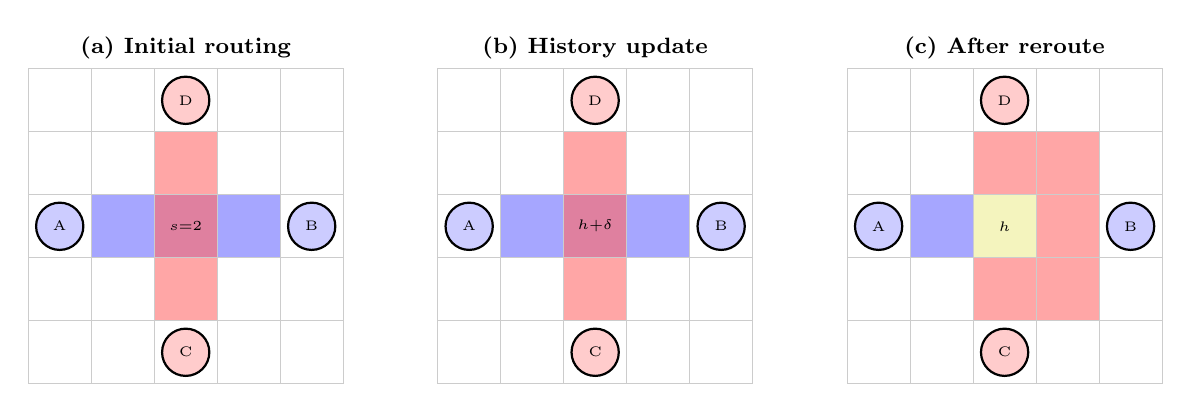
\begin{tikzpicture}[
    cell/.style={minimum size=8mm, draw=gray!40, inner sep=0pt},
    node/.style={circle, draw, thick, minimum size=6mm, font=\scriptsize},
    route1/.style={fill=blue!35},
    route2/.style={fill=red!35},
    conflict/.style={fill=purple!50},
    history/.style={fill=yellow!30},
    font=\footnotesize,
]

% --- Panel (a): Initial routes overlap ---
\begin{scope}[shift={(0,0)}]
\node[font=\footnotesize\bfseries, anchor=south] at (1.6, 3.6) {(a) Initial routing};

% Grid
\foreach \x in {0,...,4} {
    \foreach \y in {0,...,4} {
        \node[cell] at (\x*0.8, \y*0.8) {};
    }
}

% Route 1: A to B (horizontal through middle)
\foreach \x in {1,2,3} {
    \node[cell, route1] at (\x*0.8, 2*0.8) {};
}
% Route 2: C to D (vertical through middle)
\foreach \y in {1,2,3} {
    \node[cell, route2] at (2*0.8, \y*0.8) {};
}
% Conflict cell
\node[cell, conflict] at (2*0.8, 2*0.8) {};
\node[font=\tiny, black] at (2*0.8, 2*0.8) {$s{=}2$};

% Endpoints
\node[node, fill=blue!20] at (0, 2*0.8) {\tiny A};
\node[node, fill=blue!20] at (4*0.8, 2*0.8) {\tiny B};
\node[node, fill=red!20] at (2*0.8, 0) {\tiny C};
\node[node, fill=red!20] at (2*0.8, 4*0.8) {\tiny D};
\end{scope}

% --- Panel (b): History penalty applied ---
\begin{scope}[shift={(5.2,0)}]
\node[font=\footnotesize\bfseries, anchor=south] at (1.6, 3.6) {(b) History update};

\foreach \x in {0,...,4} {
    \foreach \y in {0,...,4} {
        \node[cell] at (\x*0.8, \y*0.8) {};
    }
}

% Same routes
\foreach \x in {1,2,3} {
    \node[cell, route1] at (\x*0.8, 2*0.8) {};
}
\foreach \y in {1,2,3} {
    \node[cell, route2] at (2*0.8, \y*0.8) {};
}
% Conflict cell with history
\node[cell, conflict] at (2*0.8, 2*0.8) {};
\node[font=\tiny, black] at (2*0.8, 2*0.8) {$h{+}\delta$};

% Endpoints
\node[node, fill=blue!20] at (0, 2*0.8) {\tiny A};
\node[node, fill=blue!20] at (4*0.8, 2*0.8) {\tiny B};
\node[node, fill=red!20] at (2*0.8, 0) {\tiny C};
\node[node, fill=red!20] at (2*0.8, 4*0.8) {\tiny D};
\end{scope}

% --- Panel (c): After reroute ---
\begin{scope}[shift={(10.4,0)}]
\node[font=\footnotesize\bfseries, anchor=south] at (1.6, 3.6) {(c) After reroute};

\foreach \x in {0,...,4} {
    \foreach \y in {0,...,4} {
        \node[cell] at (\x*0.8, \y*0.8) {};
    }
}

% History ghost on center cell (drawn after routes so label is visible)
% Route 1: same horizontal
\foreach \x in {1,3} {
    \node[cell, route1] at (\x*0.8, 2*0.8) {};
}
% Center cell: route1 passes through but history remains visible
\node[cell, fill=blue!15!yellow!30] at (2*0.8, 2*0.8) {};
\node[font=\tiny, black] at (2*0.8, 2*0.8) {$h$};

% Route 2: detours around conflict
\node[cell, route2] at (2*0.8, 0.8) {};
\node[cell, route2] at (3*0.8, 0.8) {};
\node[cell, route2] at (3*0.8, 1.6) {};
\node[cell, route2] at (3*0.8, 2.4) {};
\node[cell, route2] at (2*0.8, 2.4) {};

% Endpoints
\node[node, fill=blue!20] at (0, 2*0.8) {\tiny A};
\node[node, fill=blue!20] at (4*0.8, 2*0.8) {\tiny B};
\node[node, fill=red!20] at (2*0.8, 0) {\tiny C};
\node[node, fill=red!20] at (2*0.8, 4*0.8) {\tiny D};
\end{scope}

\end{tikzpicture}
\caption{PathFinder negotiation resolving a routing conflict. (a)~Two routes
(blue: A$\to$B, red: C$\to$D) share a cell ($s=2$). (b)~The shared cell
receives a history penalty $h + \delta$, increasing its cost. (c)~On the next
iteration, the lower-weight route (red) detours around the now-expensive cell,
eliminating the conflict.}
\label{fig:pathfinder}
\end{figure}

% ────────────────────────────────────────────────────────────────
\section{Scoring}

The composite score combines four normalized metrics:

\begin{table}[h]
\centering
\begin{tabular}{@{}lll@{}}
\toprule
Metric & Definition & Ideal \\
\midrule
Path efficiency $s_\text{pe}$ & $\frac{1}{|E'|}\sum_{e \in E'} \frac{d_\text{manhattan}(e)}{|\gamma(e)|}$ & 1.0 \\[4pt]
Accessibility $s_\text{acc}$ & $|E'| / |E|$ & 1.0 \\[4pt]
Congestion $s_\text{cong}$ & $1 / \max_p s(p)$ & 1.0 \\[4pt]
Void ratio $s_\text{vr}$ & $1 - \frac{|r_\text{void} - 0.2|}{0.2}$ & 1.0 \\
\bottomrule
\end{tabular}
\caption{Scoring metrics. Each is in $[0, 1]$; the composite is their mean.}
\end{table}

The void ratio metric penalizes deviation from $\sim$20\% empty space, encoding
the observation that believable layouts are neither packed solid nor mostly
empty.

% ────────────────────────────────────────────────────────────────
\section{Implementation}

Ogun is implemented in Rust (edition 2024, MSRV 1.85) with the following
performance-critical design choices:

\paragraph{Struct-of-arrays (SoA) layout.} Placed node coordinates are stored as separate
\texttt{Vec<f32>} arrays (x, y, radius) rather than an array of structs,
enabling SIMD auto-vectorization of the repulsion loop.

\paragraph{Parallel evaluation.} For large grids ($W \times H \times
n_\text{placed} \geq 500{,}000$), utility evaluation is parallelized across
rows using Rayon.

\paragraph{Buffer reuse.} Dijkstra distance/predecessor arrays and BFS queues
are allocated once and reused across all routing calls.

\paragraph{Determinism.} All randomness flows through a single
\texttt{ChaCha8Rng} seeded from the configuration. Same input $=$ same output.

\subsection{Benchmarks}

\begin{table}[h]
\centering
\begin{tabular}{@{}rrrr@{}}
\toprule
Nodes & Grid & Time & Speedup vs.\ naive \\
\midrule
50 & $100 \times 100$ & 44\,ms & 3.2$\times$ \\
100 & $250 \times 110$ & 323\,ms & 5.0$\times$ \\
200 & $250 \times 250$ & 1.28\,s & 9.5$\times$ \\
500 & $500 \times 500$ & 11.3\,s & 24.8$\times$ \\
\bottomrule
\end{tabular}
\caption{Release-mode benchmarks. Naive baseline uses AoS layout, no cutoff,
no parallelism, no buffer reuse.}
\end{table}

% ────────────────────────────────────────────────────────────────
\section{Application: Procedural City Generation}

Figure~\ref{fig:city} shows a city layout generated by
Oku\footnote{\url{https://github.com/EliasVahlberg/oku}}, a procedural city
generator built on Ogun. Graph nodes represent buildings (residential,
commercial, military, religious); edges represent infrastructure demands (roads,
utilities). The \texttt{boundary\_affinity} kernel places military structures
near the perimeter, while \texttt{cell\_bonus} encodes zoning preferences.
Routing costs create natural road hierarchy: main arteries through low-cost
corridors, minor streets through higher-cost residential areas.

\begin{figure}[h]
\centering
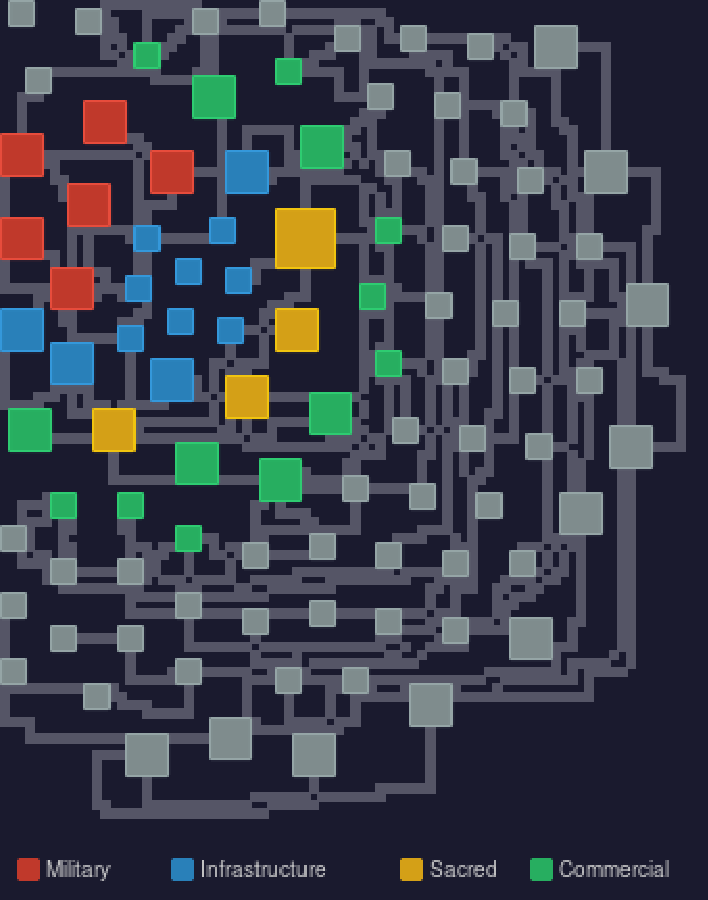
\includegraphics[width=0.55\textwidth]{city.pdf}
\caption{A procedural city layout generated by Oku using the Ogun algorithm.
Colored rectangles represent buildings of different types; gray paths are routed
roads. The layout exhibits emergent clustering and road hierarchy from the
potential function and negotiation routing.}
\label{fig:city}
\end{figure}

% ────────────────────────────────────────────────────────────────
\section{Complexity Analysis}

Let $n = |V|$, $m = |E|$, $A = W \times H$.

\begin{table}[h]
\centering
\begin{tabular}{@{}lll@{}}
\toprule
Phase & Time & Space \\
\midrule
Utility evaluation (per node) & $O(A \cdot n)$ & $O(A)$ \\
Boltzmann sampling (per node) & $O(A)$ & $O(1)$ \\
Dijkstra routing (per edge) & $O(A \log A)$ & $O(A)$ \\
Phase 1 total & $O(n \cdot A \cdot n + m \cdot A \log A)$ & $O(A + n + m)$ \\
Phase 2 ($T$ iterations) & $O(T \cdot m \cdot A \log A)$ & $O(A + m)$ \\
Scoring & $O(m \cdot A)$ & $O(A)$ \\
\bottomrule
\end{tabular}
\caption{Asymptotic complexity. $A = W \times H$ is the grid area.}
\end{table}

The dominant cost is utility evaluation: $O(n^2 A)$ total across all nodes.
With the repulsion cutoff and Rayon parallelism, the practical constant is
small; the 500-node benchmark completes in 11.3\,s on a $500 \times 500$ grid.

% ────────────────────────────────────────────────────────────────
\section{Conclusion}

Ogun demonstrates that sequential logit dynamics provide an effective framework
for coupled placement-and-routing on 2D grids. The potential game formulation
gives a clean decomposition of placement quality into interpretable terms
(attraction, repulsion, boundary affinity, cell bonus), while the Boltzmann
parameter $\beta$ provides principled control over the optimization--exploration
tradeoff. PathFinder negotiation routing, adapted from EDA, produces emergent
road hierarchy without explicit priority assignment.

The algorithm is deterministic, domain-agnostic, and thread-safe. Its
application to procedural city generation via the Oku system demonstrates that
EDA-derived techniques transfer effectively to game content generation.

Future work includes hierarchical generation (running Ogun at district, block,
and building scales), a target convergence loop that adjusts $\beta$ to reach a
desired composite score, and functional erosion, a cascading degradation model that
transforms optimized layouts into believable ruins.

% ────────────────────────────────────────────────────────────────
\begin{thebibliography}{9}

\bibitem{blume1993}
L.~E. Blume, ``The statistical mechanics of strategic interaction,''
\emph{Games and Economic Behavior}, vol.~5, no.~3, pp.~387--424, 1993.

\bibitem{mcmurchie1995}
L.~McMurchie and C.~Ebeling, ``PathFinder: A negotiation-based
performance-driven router for FPGAs,'' in \emph{Proc.\ ACM/SIGDA FPGA},
pp.~111--117, 1995.

\bibitem{monderer1996}
D.~Monderer and L.~S. Shapley, ``Potential games,'' \emph{Games and Economic
Behavior}, vol.~14, no.~1, pp.~124--143, 1996.

\bibitem{lee1961}
C.~Y. Lee, ``An algorithm for path connections and its applications,''
\emph{IRE Trans.\ Electronic Computers}, vol.~EC-10, no.~3, pp.~346--365,
1961.

\bibitem{togelius2011}
J.~Togelius, G.~N. Yannakakis, K.~O. Stanley, and C.~Browne, ``Search-based
procedural content generation: A taxonomy and survey,'' \emph{IEEE Trans.\
Computational Intelligence and AI in Games}, vol.~3, no.~3, pp.~172--186, 2011.

\bibitem{shaker2016}
N.~Shaker, J.~Togelius, and M.~J. Nelson, \emph{Procedural Content Generation
in Games}. Springer, 2016.

\end{thebibliography}

\end{document}
